\chapter{RUMIS - Nonmonotonic Rule Mining System}\label{chap:system}

RUMIS stands for Nonmonotonic Rule Mining System which is the main tool in the current work and is exploited to revise Horn rules under the OWA. This chapter describes in details the practical implementation of theory framework presented in Chapter~\ref{chap:frame} and uses background definitions in Chapter~\ref{chap:back}. Organization of the chapter is as follows, first, an overview of the RUMIS is discussed. Second, the implementations of main components in the system are presented. Finally, we talk about usage of the system.

\section{System Overview}
\label{sec:overview}

There are six components in RUMIS as presented in Figure~\ref{system_overview} with arrows indicating the data flow from input to output. RUMIS mines the nonmonotonic rules from the original graph in the following steps:

\begin{itemize}
\item In (1), a KG $\cG$ as an input is passed to RUMIS. It is then stored and indexed into the system by Component 1 which is exploited to speed up computation in the next steps.
\item In (2), Horn rules are mined by Component 2 from facts indexed into RUMIS.
\item In (3), normal and abnormal sets are found by Component 3 based on KG $\cG$ and mined Horn rules in the previous step.
\item With normal and abnormal sets known for each Horn rule, (4) represents for finding exception witness sets in Component 4.
\item In (5) and (6), exception candidates are ranked in Component 6 using a measure plugged by Component 5. RUMIS allocates a separate component for measure plugin to flexibly extend ranking criteria in the future.
\item In (7), after being ranked, the best revision for each Horn rule is added to the output of RUMIS.
\end{itemize}

\begin{figure}[ht]
\centering
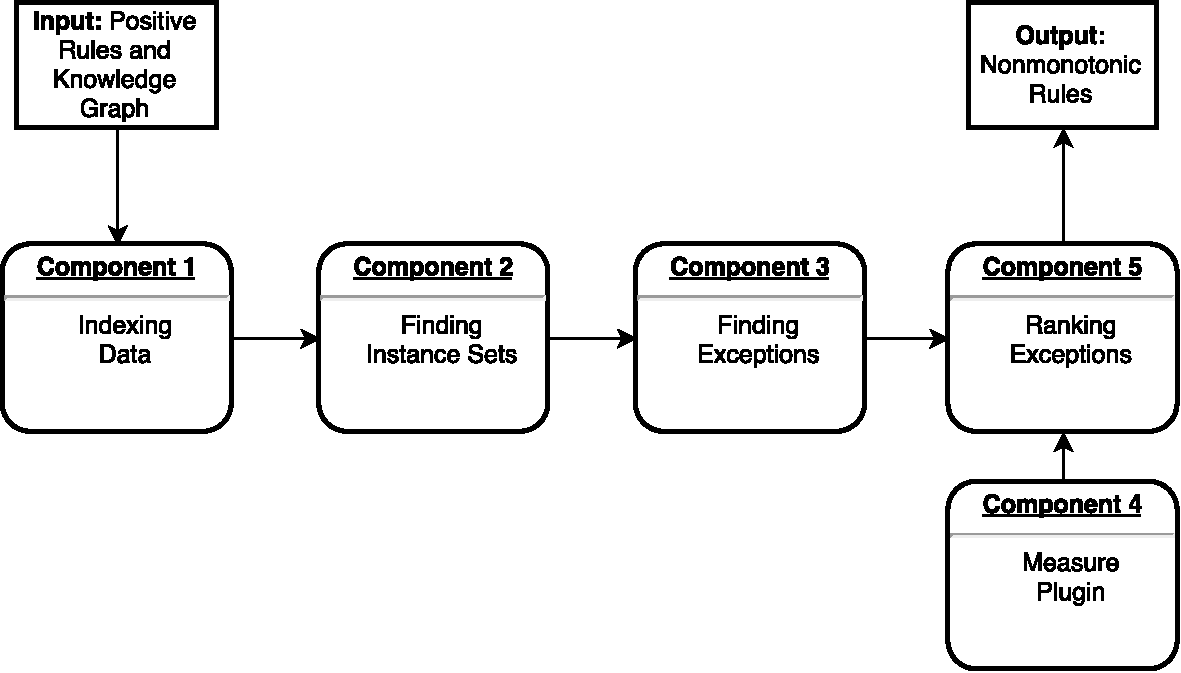
\includegraphics[width=0.85\textwidth]{figures/system_overview}
\caption{Components of RUMIS}
\label{system_overview}
\end{figure}

\section{Implementation}

In this section, the main components mentioned in Section~\ref{sec:overview} are described in details. To simplify the problem of \textit{language bias}, the implementation of RUMIS only takes the following positive rule form into consideration:

\begin{equation}
r2: h(X, Z) \leftarrow p(X, Y), q(Y, Z)
\label{form2}
\end{equation}

Where $h$, $p$, $q$ are binary predicates from KG $\cG$, these notations and the form~\ref{form2} ($r2$) are used in the rest of this thesis.

\subsection{Data Indexing}
\label{data_indexing}

\begin{figure}[ht]
\centering
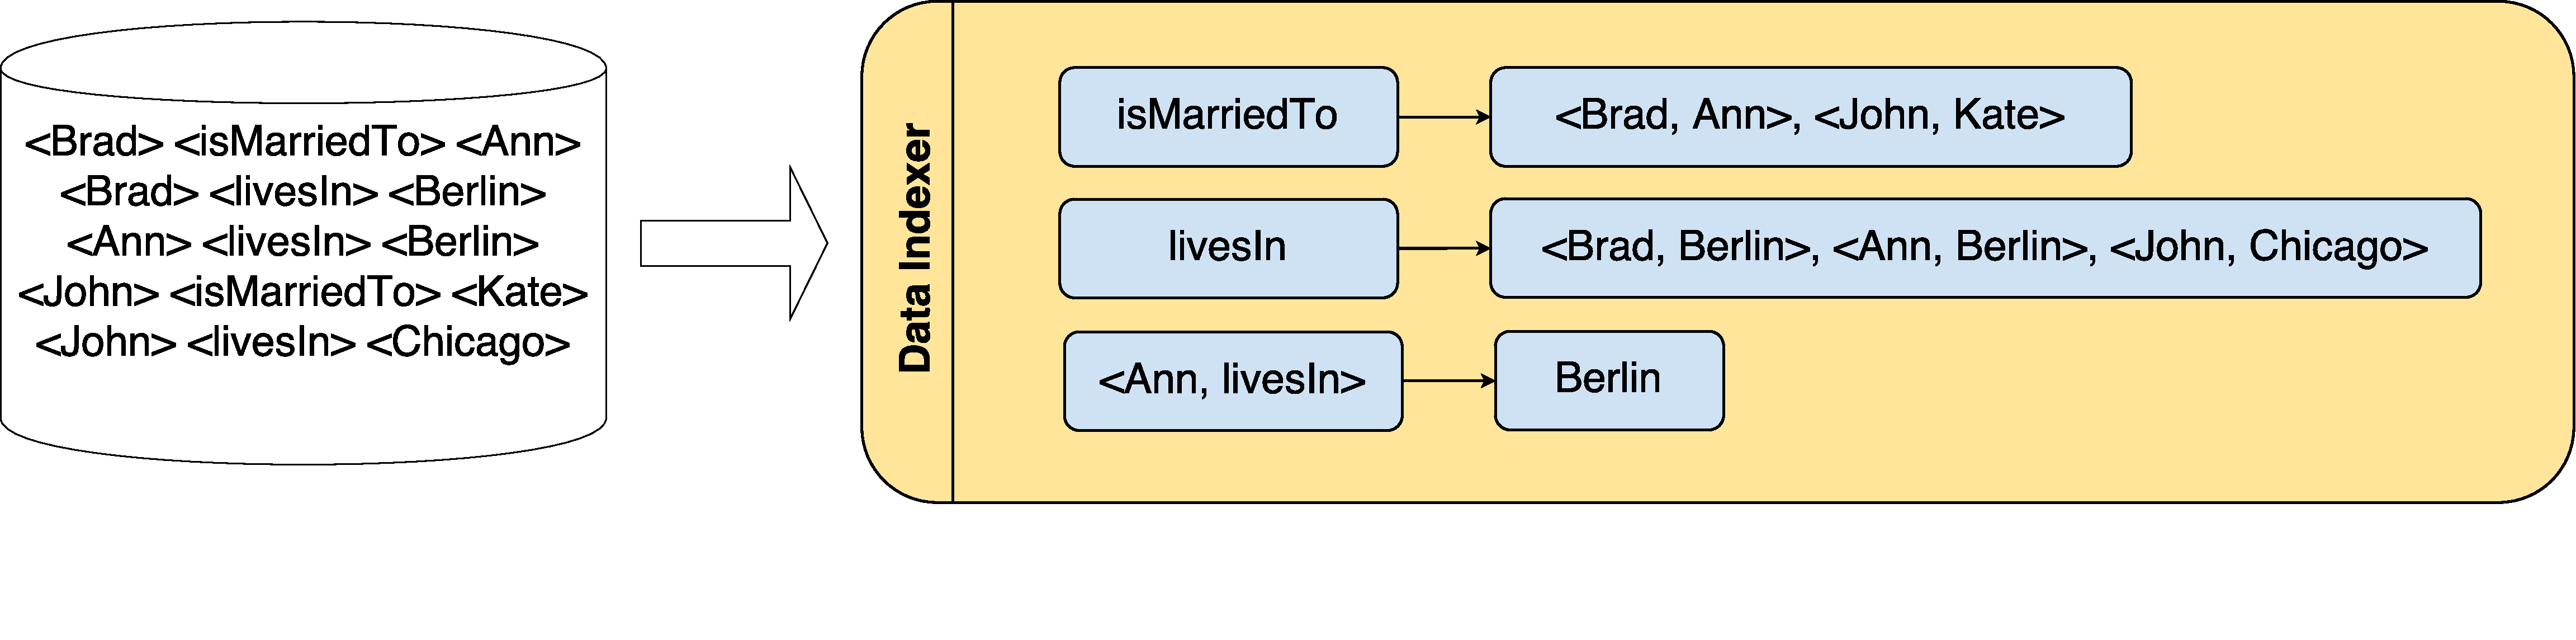
\includegraphics[width=1.0\textwidth]{figures/data_indexing}
\caption{RUMIS Data Indexer}
\label{data_indexing}
\end{figure}

Since the KG $\cG$ can be huge, it takes a long time to find (ab)normal instances and exception witness sets of a positive rule. To overcome this, data indexing is taken into consideration to speed up processing data. In a traditional search engine, terms such as words, n-grams are indexed into the system and their corresponding posting lists~\cite{ref47} are a collection of documents containing them. The same intuition can be applied to relational setting in the current work. Indeed, RUMIS treats every fact as a document and the terms can be subjects, predicates, objects or some combinations of them.

To be specific, Figure~\ref{data_indexing} illustrates data indexed from part of KG in Figure~\ref{fig1.1}. In the figure, based on the index, if predicate \textit{isMarriedTo} is given, we can find set of subject-object pairs corresponding to this relation, i.e., \textit{$<$Brad, Ann$>$} and \textit{$<$John, Kate$>$}. Besides, objects can be found if we have at hand their corresponding subjects and relations. For example, we can get ``Berlin" as an answer to the question: ``Where does Ann live" based on data indexing illustrated in the Figure~\ref{data_indexing}. In this example, the term is the combination of subjects and predicates. More formally, Data Indexing provides the following functions that are exploited in the rest components:

\begin{itemize}
\item \textit{getPredicateSubjectSet($\cG$, object):} This function returns a set of predicate-subject pairs corresponding to a given \textit{object} in KG $\cG$.
\item \textit{getPredicateSet($\cG$, subject, object):} A set of predicates corresponding to input \textit{subject, object} entities are found in this function.
\item \textit{getSubjectSet($\cG$, predicate, object):} A set of subjects are an output for given \textit{predicate, object} based on this function.
\item \textit{getSubjectObjectSet($\cG$, predicate):} This function is to find a set of subject-object pairs if we have \textit{predicate} at hand as a parameter.
\end{itemize}

\subsection{Positive Rule Mining}

Positive Rule Mining finds Horn rule $r2$ in the form~\ref{form2} with high \textit{absolute support}. The way how this works is illustrated in Algorithm~\ref{algo1} with the following steps. First, in line 1, \textit{absSupp} is created with the aim to store absolute support of positive rules. More specifically, $absSupp[hpq]$ is the absolute support of rule \textit{r2}. Second, for each triple \textit{$<$Y q Z$>$} from KG $\cG$, a set of pairs \textit{X, p} are found such that \textit{$<$X p Y$>$} is in $\cG$ (line 2 and 3). Command in line 3 is executed using \textit{getPredicateSubjectSet} function in Data Indexing component. Third, from line 5 to 6, with \textit{X, Z} found in the previous step, RUMIS searches for every relation $h$ s.t. \textit{$<$X h Z$>$} is in $\cG$. At this point, it is guaranteed that \textit{h(X, Z), p(X, Y), q(Y, Z)} holds true. After that, in line 7, absolute support of the rule \textit{r2} is increased by $1$. Finally, all rules are sorted in decreasing order of absolute support (line 11).

\IncMargin{1.5em}
\begin{algorithm}[H]
\DontPrintSemicolon
\SetAlgoLined
\SetKwInOut{Input}{Input}\SetKwInOut{Output}{Output}
\Input{KG $\cG$}
\Output{Set of positive rules with the same form as $r2$}
\BlankLine
$absSupp \leftarrow \{\}$\\
\BlankLine
\ForEach{Triple $YqZ$ in $\cG$} {
    \BlankLine
	$pXSet \leftarrow getPredicateSubjectSet(\cG, Y)$\\
	\ForEach{Pair $pX$ in $pXSet$} {
		$hSet \leftarrow getPredicateSet(\cG, X, Z)$\\
		\ForEach{Predicate $h$ in $hSet$} {
			$absSupp[hpq]++$\\
		}
	}
}
\BlankLine
Sort $hpq$ according to deacreasing order of $absSupp[hpq]$\\
\Return $absSupp$\\
\caption{Positive Rule Mining}
\label{algo1}
\end{algorithm}
\DecMargin{1.5em}

\subsection{Normal and Abnormal Set Mining}

This component explores normal and abnormal sets of rule \textit{r2} in Algorithm~\ref{algo2} as follows. First, in lines 1 and 2, (ab)normal sets are created. Second, for each pair \textit{Y, Z} s.t. \textit{$<$Y q Z$>$} is in $\cG$, a set of $X$ in the fact \textit{$<$X p Y$>$} from the KG are found based on Data Indexing component (line 3 to 5). At this point, it is guaranteed that \textit{X, Y, Z}  fulfills the body of rule \textit{r2}. Finally, for every $X$ found in the previous step, \textit{$<$X h Z$>$} is verified to be in the the KG or not. If it is in $\cG$, \textit{$<$X Z$>$} is added to the normal set, otherwise it is added to the abnormal set.

\IncMargin{1.5em}
\begin{algorithm}[H]
\DontPrintSemicolon
\SetAlgoLined
\SetKwInOut{Input}{Input}\SetKwInOut{Output}{Output}
\Input{KG $\cG$, $h$, $p$, $q$ predicates in the rule $r2$}
\Output{Normal and abnormal sets of the rule $r2$}
\BlankLine
$NS \leftarrow \{\}$\\
$ABS \leftarrow \{\}$\\
$YZSet \leftarrow getSubjectObjectSet(\cG, q)$\\
\BlankLine
\ForEach{Pair $YZ$ in $YZSet$} {
    \BlankLine
	$XSet \leftarrow getSubjectSet(\cG, p, Y)$\\
	\ForEach{$X$ in $XSet$} {
	\uIf{$XhZ$ is in $\cG$} {
		Add $XZ$ to $NS$\\
	}
	\uElse {
		Add $XZ$ to $ABS$\\
	}
	}
}
\BlankLine
\Return $NS$ and $ABS$\\
\caption{Normal and Abnormal Set Mining}
\label{algo2}
\end{algorithm}
\DecMargin{1.5em}

\subsection{Exception Witness Set Mining}

Binary predicate exception candidates of positive rules \textit{r2} are an output for Algorithm~\ref{algo3}. More specifically, our goal is to find exceptions with the form \textit{e(X, Z)}, they are then inserted to the body of $r2$ to get its revised rule \textit{h(X, Z) :- p(X, Y), q(Y, Z), not e(X, Z)}. Similarly, unary exceptions \textit{e(X)} or \textit{e(Z)} can be mined in an equivalent way with binary ones. As regards Algorithm~\ref{algo3}, there are several steps as follows, first, normal and abnormal instance sets are found from Algorithm~\ref{algo2} in line 1 and 2. In addition, $EWS+$ and $EWS-$ (i.e., set of relations between \textit{$<$X Z$>$} in the abnormal and normal sets, resp.) are created (line 3 and 4). Second, for every pair \textit{$<$X Z$>$} in the abnormal set, all relations between them are added to the $EWS+$ (line 5 to 8). After that, similar stage is applied for $EWS-$ from line 9 to 12. Finally, exception witness set $EWS$ is calculated as the difference between $EWS+$ and $EWS-$ (line 13).

\IncMargin{1.5em}
\begin{algorithm}[H]
\DontPrintSemicolon
\SetAlgoLined
\SetKwInOut{Input}{Input}\SetKwInOut{Output}{Output}
\Input{KG $\cG$, $h$, $p$, $q$ predicates of the rule $r2$}
\Output{Exception witness set of the rule $r2$}
\BlankLine
$NS \leftarrow getNormalSet(\cG, h, p, q)$\\
$ABS \leftarrow getAbnormalSet(\cG, h, p, q)$\\
$EWS+ \leftarrow \{\}$\\
$EWS- \leftarrow \{\}$\\
\BlankLine
\ForEach{Pair $XZ$ in $ABS$} {
	$pSet \leftarrow getPredicateSet(\cG, X, Z)$\\
	$EWS+$ $\leftarrow$ $EWS+$ $\cup$ $pSet$\\
}
\ForEach{Pair $XZ$ in $NS$} {
	$pSet \leftarrow getPredicateSet(\cG, X, Z)$\\
	$EWS-$ $\leftarrow$ $EWS-$ $\cup$ $pSet$\\
}
$EWS$ $\leftarrow$ $EWS+$ $\setminus$ $EWS-$\\
\Return $EWS$\\
\caption{Exception Witness Set Mining}
\label{algo3}
\end{algorithm}
\DecMargin{1.5em}

\subsection{Measure Plugin}

To be easy to plugin and test another rule quality criteria, the measure plugin is designed as a separate component. There are two main measures in the current implementation: confidence and conviction. While the former is a good choice for descriptive purpose, its predictive quality is not as good as that of the latter~\cite{ref46}. Since the main concern of this thesis is to revise Horn rules and subsequently predict accurate facts to expand the original KG, conviction is the main measure in RUMIS.

\subsection{Exception Ranking}
\label{intuition_er}

Figure~\ref{pm_ranking} shows some arrows representing for the communications between different parts in (O)PM ranking. In general, the communications express the intuition for the ranking as follows.

\begin{itemize}
\item From a KG $\cG$ and a set of Horn rules, EWS mining is executed to find exception candidates for each Horn rule in (1).
\item (2) shows that some rules with exceptions (revisions) are used to infer new facts from the original KG. The strategy how to select the revisions is the difference between PM and OPM ranking.
\item $\cG'$, i.e., original KG $\cG$ with new predicted facts, is exploited to rank exceptions for each Horn rule in (3). The combination of steps (2) and (3) describes the interaction of different rules, i.e, facts generated by other revisions are taken into account to measure quality of a particular nonmonotonic rule. That is also the intuition of (O)PM ranking.
\item (4) is a process that exceptions are ranked by Component 5, the best exception is chosen to be added in final revision set.
\end{itemize}

\begin{figure}[ht]
\centering
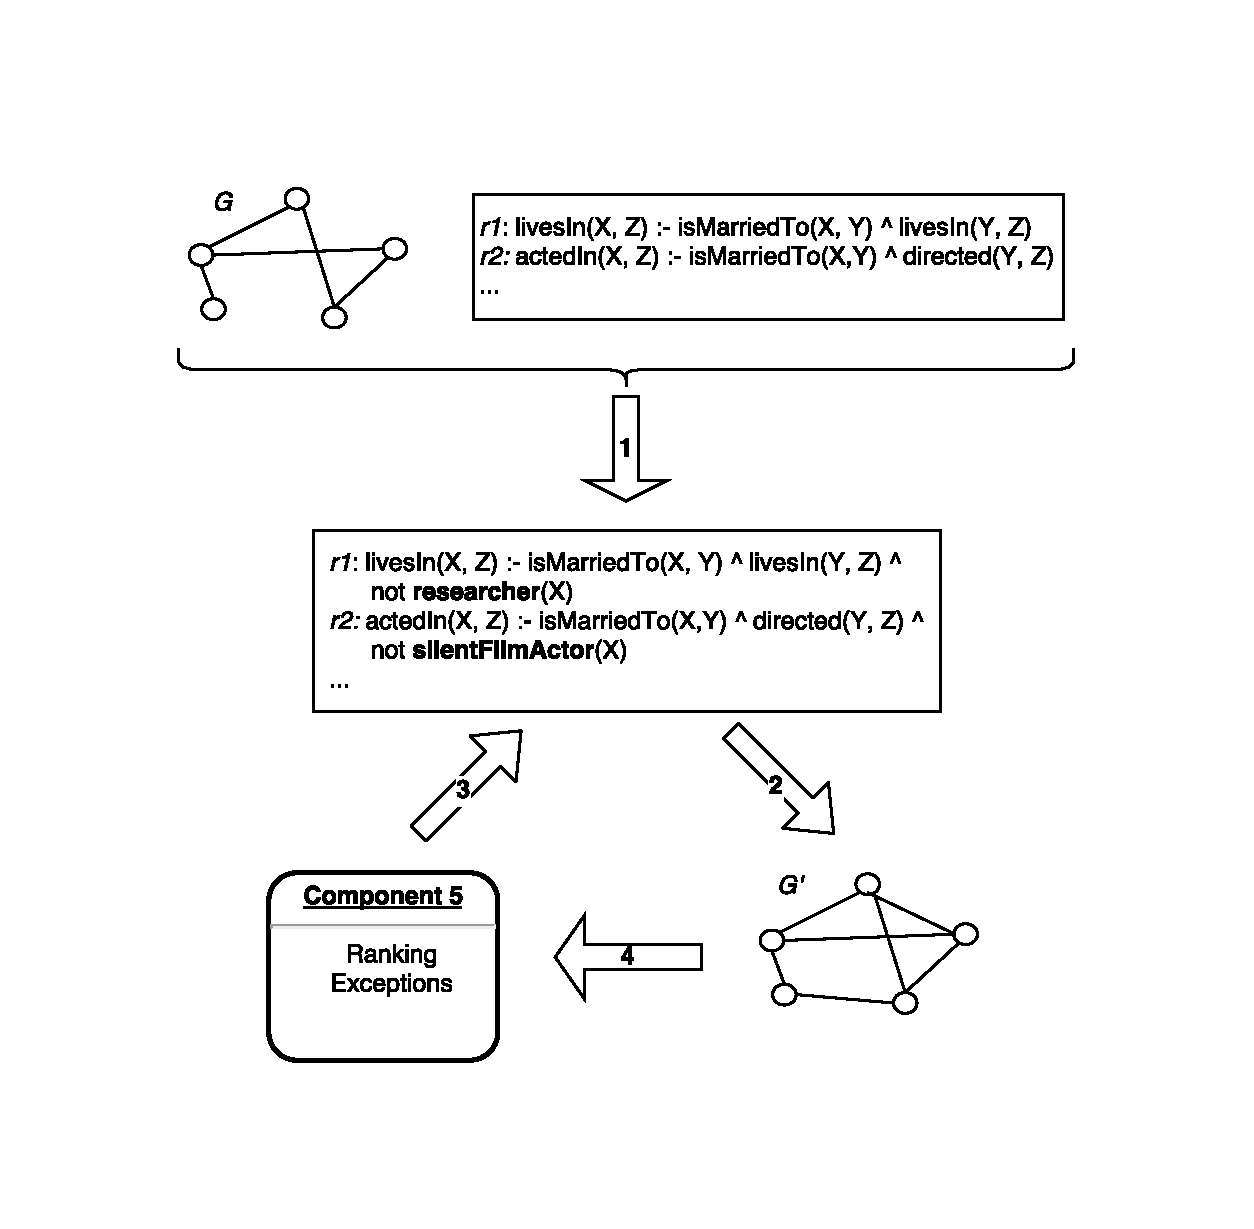
\includegraphics[width=1.0\textwidth]{figures/ranking}
\caption{(Ordered) Partial Materialization Ranking}
\label{pm_ranking}
\end{figure}

\textit{Definition 1.[plan to move this definition to background section]} Safely predicted facts of $r$ w.r.t. KG $\cG$ are all new facts produced by $r$ and not by any revision of $r$ constructing by adding an exception candidate to the rule body. [Give an example, ...]

\textbf{PM Ranking.} The Algorithm~\ref{bf_pm_ranking_algo} describes the intuition for PM ranking step by step. In line 1, a set of revised rules are initialized as an empty set. After that, for each positive rule $r$ in $R_H$, we clone original KG $\cG$ to a new one ($\cG'$), then all other rules in $R_H$ are exploited to generate their safely predicted facts which are subsequently indexed to $\cG'$ (line 2 to 6). RUMIS is conservative in producing new facts since the system applies revisions to $\cG$ instead of $\cG'$ in every iteration. This eliminates the cases that wrong facts introduce many incorrect ones in the future process. Next, in line 7 and 8, based on the new KG, exceptions of $r$ are ranked and the best revision is added to $R_{NM}$. Finally, we return $R_{NM}$ as a result for the algorithm.

\IncMargin{1.5em}
\begin{algorithm}[H]
\DontPrintSemicolon
\SetAlgoLined
\SetKwInOut{Input}{Input}\SetKwInOut{Output}{Output}
\Input{KG $\cG$, set of positive rules $\cR_{H}$}
\Output{Set of best revisions $R_{NM}$ for the given positive rules $R_H$}
\BlankLine
$R_{NM} \leftarrow \{\}$\\
\BlankLine
\ForEach{Rule $r$ in $R_H$} {
	$\cG' \leftarrow \cG$\\
	\ForEach{Rule $r''$ in $R_H$, $r''$ is different from $r$} {
		Generate safely predicted facts of $r''$ w.r.t. $\cG$ then index these facts to $\cG'$\\
	}
	Rank exceptions of $r$ based on $\cG'$, choose $r'$ as the best revision of $r$\\
	Add $r'$ to $R_{NM}$\\
}
\Return $R_{NM}$\\
\caption{PM Ranking}
\label{bf_pm_ranking_algo}
\end{algorithm}
\DecMargin{1.5em}

\textbf{OPM Ranking.} This function (Algorithm~\ref{opm_ranking_algo}) is similar to PM ranking, the major difference is the way how to select revisions to expand KG $\cG'$. In details, there are several steps in the algorithm as follows. From line 1 to 2, $\cG$ is cloned to $\cG'$ and $R_{NM}$ is created as an empty rule set. The line 1 reflects the contrast between Algorithm~\ref{bf_pm_ranking_algo} and~\ref{opm_ranking_algo} since the latter executes cloning only one time. In the next step, all the Horn rules are then sorted in decreasing order of conviction measure (line 3). Similar to PM, for each Horn rule $r$ in $R_H$ (line 4), OPM ranking chooses the best revision of $r$ based on $G'$ for the final result (line 5 and 6). After that, in line 7, safely new facts are predicted to update KG $\cG'$.

Intuitively, all safely predicted facts from previous rules w.r.t. $\cG$ are added to $\cG'$ which is exploited to assess quality of $r$. In OPM ranking, the order of Horn rules regarding the conviction matters, i.e., the higher conviction quality of an Horn rule, the more important impact it plays on the other rules. In other words, OPM is more conservative than PM ranking, only safely predicted facts of better Horn rules may be taken into account to revise a particular one.

\IncMargin{1.5em}
\begin{algorithm}[H]
\DontPrintSemicolon
\SetAlgoLined
\SetKwInOut{Input}{Input}\SetKwInOut{Output}{Output}
\Input{KG $\cG$, set of positive rules $\cR_{H}$}
\Output{Set of best revisions $R_{NM}$ for the given positive rules $R_H$}
\BlankLine
$\cG' \leftarrow \cG$\\
$R_{NM} \leftarrow \{\}$\\
Sort all rules in $R_H$ according to the decreasing order of conviction\\
\BlankLine
\ForEach{Rule $r$ in $R_H$} {
	Rank exceptions of $r$ based on $\cG'$, choose $r'$ as the best revision of $r$\\
	Add $r'$ to $R_{NM}$\\
	Generate safely predicted facts of $r$ w.r.t. $\cG$ then index these facts to $\cG'$\\
}
\Return $R_{NM}$\\
\caption{OPM Ranking}
\label{opm_ranking_algo}
\end{algorithm}
\DecMargin{1.5em}

\section{Optimization}

To accomplish the Algorithm~\ref{bf_pm_ranking_algo}, cloning KG $\cG$ and indexing safely predicted facts are executed $|R_H|$ and $|R_H|^2$ times, resp. Since the number of facts in $\cG$ and positive rules can be large, this algorithm takes long time to process, and thus, is not scalable. We need to optimize it s.t. cloning KG should not be called many times because copying from a KG to a new one is time consuming. Besides, accessing to Data Indexer should be restricted to speed up PM ranking. This is a motivation for introducing Algorithm~\ref{pm_ranking} as a refined algorithm for PM ranking which is implemented in the following steps.

In lines 1 and 2 of the Algorithm~\ref{pm_ranking}, we clone an original graph $\cG$ to $\cG'$ and create empty nonmonotonic rule set $R_{NM}$. After that, from line 3 to 5, for every Horn rule $r$ in $R_H$, its safely predicted facts are added to $\cG'$ using Data Indexing component. 

Now RUMIS is ready for refined PM ranking, in line 7, for each Horn rule $r$, indexes of its safely predicted facts are removed from $\cG'$. This step is to make sure that safely predicted facts of all other rules ($r$ excluded) are exploited to determine quality of $r$ (line 8). Thanks to this, the interaction between nonmonotonic rules are taken into consideration for the ranking. After that, the best revision of $r$ is added to the final result in line 9. Line 10 shows a step that undoes what is done in line 7, i.e., safely predicted facts of rule $r$ based on $\cG$ is added to $\cG'$ again. This guarantees the same setting in the next iteration can be processed with a new rule.

\IncMargin{1.5em}
\begin{algorithm}[H]
\DontPrintSemicolon
\SetAlgoLined
\SetKwInOut{Input}{Input}\SetKwInOut{Output}{Output}
\Input{KG $\cG$, set of positive rules $\cR_{H}$}
\Output{Set of best revisions $R_{NM}$ for the given positive rules $R_H$}
\BlankLine
$\cG' \leftarrow \cG$\\
$R_{NM} \leftarrow \{\}$\\
\BlankLine
\ForEach{Rule $r$ in $R_H$} {
	Generate safely predicted facts of $r$ w.r.t. $\cG$ then index these facts to $\cG'$\\
}
\BlankLine
\ForEach{Rule $r$ in $R_H$} {
	Generate safely predicted facts of $r$ w.r.t. $\cG$ then remove these facts' indexes from $\cG'$\\
	Rank exceptions of $r$ based on $\cG'$, choose $r'$ as the best revision of $r$\\
	Add $r'$ to $R_{NM}$\\
	Generate safely predicted facts of $r$ w.r.t. $\cG$ then index these facts to $\cG'$ (undoes step in line 7)\\
}
\Return $R_{NM}$\\
\caption{PM Ranking}
\label{pm_ranking_algo}
\end{algorithm}
\DecMargin{1.5em}

With the optimized algorithm, we only need $O(|R_H|)$ times for indexing new predicted facts and one time for cloning KG. This is a significant improvement compared with the original version. The difference can be clearly seen if the KG is large and we have a lot of rules to communicate each other.

\section{Usage}

RUMIS~\footnote{\url{https://github.com/htran010589/nonmonotonic-rule-mining}} is developed and currently tested in Linux, we may extend it to Windows in the future. Besides, Java 8 should be installed before running the tool and DLV~\footnote{\url{http://www.dlvsystem.com/html/DLV_User_Manual.html}} is necessary for conducting experiment. In this section, the setting and command line interface of RUMIS are introduced, after that, features of the system are described in details.

\subsection{Setting}

\textbf{DLV.} This tool is used to extend a KG given a set of Horn or nonmonotonic rules at hand. RUMIS exploits DLV in its experiment function, i.e, a feature of RUMIS for evaluating result.

\textbf{Predicate Ratio and Learning KG.} RUMIS provides a function for creating a learning KG based on a predicate ratio. For example, given the KG and 0.8 as the ratio, then 80\% facts of every binary predicate are retained in the learning KG. The original KG is called the approximated ideal one.

\textbf{Working Folder.} Working folder is a location for experiment where we have learning and approximated ideal KGs in SPO format (\textit{training.data.txt} and \textit{ideal.data.txt}, resp.), positive rule and sampled positive rule files (\textit{horn-rules.txt} and \textit{selected.horn-rules.txt}, resp.) in format~\ref{form2}. Besides, DLV binary file\footnote{\url{http://www.dlvsystem.com/files/dlv.x86-64-linux-elf-static.bin}} should be downloaded and renamed to \textit{dlv.bin} in this folder. The \textit{selected.horn-rules.txt} containing a subset of rules in \textit{horn-rules.txt}, it is only necessary if we want to revise some rules in this file.

\subsection{Command Line Options}

Users can choose some of the following options to get a suitable mode for RUMIS:

\begin{itemize}
\item \textit{-d:} This flag is to enable DLV in order to extend KG.
\item \textit{-e=[execution function]:} This requires a string as a function for execution, i.e., \textit{new, pos, neg, exp} are corresponding to creating a new learning KG, positve and nonmonotonic rule mining and conducting experiment, resp.
\item \textit{-f=[working folder path]:} This requires a string as an experiment folder path.
\item \textit{-h:} This is the command line interface description.
\item \textit{-l=[KG file path]:} This requires a string as a KG file path in SPO format.
\item \textit{-o=[predicate ratio]:} This requires a percentage as a predicate ratio to create a new learning KG.
\item \textit{-p=[Horn rule file path]:} This requires a string as an Horn rule file path in format~\ref{form2}.
\item \textit{-r=[ranking]:} This requires an integer as a ranking type, i.e., 0, 1, 2 for Naive, PM, OPM ranking, resp.
\item \textit{-s:} This flag is to enable sampling positive rules.
\item \textit{-t=[number of top Horn rules]:} This requires an integer as a number of positive rules with top absolute support.
\end{itemize}

\subsection{Usage Description}

First of all, please download the repository\footnote{\url{https://github.com/htran010589/nonmonotonic-rule-mining}}, and then uncompress \textit{data/sample.imdb.txt.zip} to get \textit{sample.imdb.txt} file. In the next step, the repository folder should be located: \textit{\$ cd nonmonotonic-rule-mining}. Now the preparation is finished, and we are ready to describe the main features of RUMIS in details.

\textbf{Generating Learning KG.} Please generate the learning data in the SPO format with the following command: \textit{\$ java -jar rumis-1.0.jar -e=new -l=[path to KG file] -o=[ratio] 1$>$[training KG file path]}.

\textit{Example.} A learning KG of the IMDB sample dataset can be generated with predicate ratio being 80\%: \textit{\$ java -jar rumis-1.0.jar -e=new -l=data/sample.imdb.txt -o=0.8 1$>$training.sample.imdb.txt}. Then \textit{training.sample.imdb.txt} file is the learning KG that we want to generate.

\textbf{Horn Rule Mining.} Please run the Horn rule mining with the following command: \textit{\$ java -jar rumis-1.0.jar -e=pos -l=[path to KG file]}. This will generate two files, \textit{horn-rules.txt} for the positive rules and \textit{horn-rules-stats.txt} with the presence of \textit{absolute support}. Both rules in two files are sorted by decreasing order of the support measure.

\textit{Example.} Please run the following command for executing IMDB Horn rule mining: \textit{\$ java -jar rumis-1.0.jar -e=pos -l=data/sample.imdb.txt}. Two generated files horn-rules.txt and horn-rules-stats.txt can be seen in the same folder with RUMIS jar file.

\textbf{Nonmonotonic Rule Mining.} Please run the nonmonotonic rule mining with the following command: \textit{\$ java -jar rumis-1.0.jar -e=neg -p=[path to positive rule file] -l=[path to KG file] -r=[ranking option] -t=[top Horn rules]}. Revised rules can be seen from generated result file \textit{revised-rules.txt} in the same folder with RUMIS jar file. Note that \textit{horn-rules.txt} is generated by using above Horn rule mining function, or by another software. However, RUMIS currently only supports Horn rules in format~\ref{form2}.

The file \textit{revised-rules.txt} lists the revisions of Horn rules from \textit{horn-rules.txt} with the ranking option being specified in the command. Two main sections are presented in \textit{revised-rules.txt}, the first one describes exceptions ranked for each Horn rule and the second one lists final selected revisions. As regards the first section, Naive ranking subsection is always presented on top of the file, followed by [PM $|$ OPM] one if [PM $|$ OPM] is selected, resp.

Every ranking subsection contains many parts separated by a blank line, each of them describes rules with exceptions. The first line of each part is a positive rule and its measure values with the format: \textit{$<$positive rule$>$ $<$Conv$>$ $<$Conf$>$}. \textit{Conv} and \textit{Conf} are abbreviations of conviction and confidence measures, resp.

The rest of each above part is top 10 negated atoms for each Horn rule which are sorted according to the decreasing order of the positive-negative conviction (\textit{PosNegConv}) of the corresponding revision achieved by inserting the negated atom to the rule. If two revisions have the same positive-negative conviction, the one with higher conviction has a higher rank. The format for describing each negated atom with its measures is: \textit{$<$not exception$>$ $<$PosNegConv$>$ $<$Conv$>$}.

The second section of the \textit{revised-rules.txt} lists chosen revisions for all the Horn rules. They are corresponding to the best exceptions of positive rules in the subsection of given ranking option.

\textit{Example.} Please run the following command for executing IMDB nonmonotonic rule mining with OPM ranking: \textit{\$ java -jar rumis-1.0.jar -e=neg -p=horn-rules.txt -l=data/sample.imdb.txt -r=2}. One may just want to revise top 10 Horn rules with the \textit{-t} option: \textit{\$ java -jar rumis-1.0.jar -e=neg -p=horn-rules.txt -l=data/sample.imdb.txt -r=2 -t=10}.

\textbf{Experiment.} First of all, please create the working folder indicated above, and then run the following command for the experiment: \textit{java -XX:-UseGCOverheadLimit -Xmx[max memory]G -jar rumis-1.0.jar -e=exp -f=[working folder] -r=[ranking] -t=[top positive rules] -d -s 1$>$experiment.txt 2$>$log} where \textit{-XX, -Xmx, -t, -d, -s} are optional. \textit{-XX} and \textit{-Xmx} are used when we want to allocate more memory for RUMIS, and, if the \textit{-t} is not used, all the rules in \textit{horn-rules.txt} are revised. Besides, \textit{-s} option should only be added to the command if we just want to care about revisions of some selected rules in \textit{selected.horn-rules.txt} file.

The first two lines of the generated file \textit{experiment.txt} present the average conviction of selected Horn rules and their final revisions. These statistics are described in the Table 1 in the next chapter with different number of top Horn rules. Besides, the rest two parts of the file show predicates extended from the learning KG for positive and revised rules, resp. Format of every tab separated line in each part is \textit{$<$relation$>$ $<$inferred facts$>$ $<$good facts$>$ $<$other facts$>$} where \textit{inferred facts} means total number of predicted triples over the relation. Besides, \textit{good} and \textit{other facts} indicate quantity of \textit{inferred facts} that are in and not in the ideal KG, resp.

The command outputs a file \textit{encode.txt} and a DLV subdirectory in the working folder. The former is a tab separated file that maps from entities and predicates of ideal KG to their encoded IDs. The latter provides some files as follows. First, \textit{training.data.kg} is the DLV format version of \textit{training.data.txt}. Second, files \textit{chosen.rules.[naive $|$ pm $|$ opm].txt.[pos $|$ neg].[number of top rules]} list chosen rules in encoded DLV format, i.e, DLV rule format s.t. predicated and exceptions are encoded. Third, files \textit{extension.[naive $|$ pm $|$ opm].txt.[pos $|$ neg].[number of top rules]} describe KGs extended from learning data in DLV format and corresponding rules. The terms \textit{pos, neg} correspond to positive and revised rule sets which are exploited to extend KG. Finally, For each of these, there are \textit{decode, needcheck, good, conflict} extension files which present KG in SPO format, facts not in the ideal KG, facts in the ideal KG and conflicts, resp.

\textit{Example.} The working folder can be built as a directory \textit{data/experiment/IMDB} that contains all of the following files. First, please rename \textit{sample.imdb.txt} file to \textit{ideal.data.txt} in the directory. Second, please sample the learning data of the ideal KG file and get \textit{training.data.txt}. Third, one should generate \textit{horn-rules.txt} as an output of positive rule mining function applied to the learning data. If only some positive rules need to be revised, we can list them in \textit{selected.horn-rules.txt}. Finally, DLV binary file should be downloaded to the directory.

The command that executes experiment with OPM ranking and top 10 positive rules (without DLV) is: \textit{java -jar rumis-1.0.jar -e=exp -f=data/experiment/IMDB/ -r=2 -t=10 1$>$experiment.txt 2$>$log}. If we want to expand memory, enable DLV and selected rule option, the following command can be used. \textit{java -XX:-UseGCOverheadLimit -Xmx300G -jar rumis-1.0.jar -e=exp -f=data/experiment/IMDB/ -r=2 -t=10 -d -s 1$>$experiment.txt 2$>$log}.